
\defi{3.1} Para una aplicación $\phi: \pazocal{M} \rightarrow \pazocal{M}$, $P\in \pazocal{M}$ es un \textbf{punto fijo} de $\phi$ si $\phi(P) = P$; y $\pazocal{D} \subset \pazocal{M}$ es un \textbf{subconjunto invariante} de $\phi$ si $\phi(\pazocal{D}) = \pazocal{M}$.

\lema{3.2} Si $g \in \iso(\P)$ y $A \neq B$ son dos puntos fijos de $g$, entonces todo $X \in r_{AB}$ es punto fijo de $g$.


\defi{3.3} Si $g, g' \in \iso(\P)$, $g$ y $g'$ son \textbf{conjugadas}
si existe una isometría $h$ tal que $gh = hg' \iff g = hg'h^{-1}$.

\tma{3.4} Un punto $P$ es fijo de $g$ sii $h^{-1}(P)$ es un punto fijo de $g'$. Es decir

\dem{Si $h^{-1}(P)$ es punto fijo de $g'$, entonces $g'(h^{-1}(P)) = h^{-1}(P)$. Por tanto, $g(P) = hg'h^{-1}(P) = hh^{-1}(P) = P$, luego $g(P) = P$.}

\ejem{3.5} Una reflexión sobre $r$ cumple que
\begin{itemizex}
	\item $\sigma_r\circ\sigma_r = \text{id}_{\P}$ y $\sigma_r(X) = X \iff X \in r$ (\axioma{P6})
	\item $\sigma_r(H^1) = H^2$ y viceversa.
	\item $X$ y $\sigma_r(X)$ se encuentran en una recta ortogonal a $r$.
\end{itemizex} 
	 
\importante\tma{3.6} Sea $g\in \iso(\P)$ y sea $r_{AB}$. Si $A, B$ son puntos fijos en $g$, entonces o bien $g = \sigma_r$ o bien $g = \text{id}_\P$. 

\tma{3.9} Llamamos $\rho$ una \textbf{rotación} a una isometría que tiene un punto fijo $C$. Para toda recta $a$ pasando por $C$ existen dos rectas $b, b'$ únicas tales que $\rho = \sigma_b\sigma_a = \sigma_a\sigma_{b'}$.

\begin{figure}[H]
	\centering
	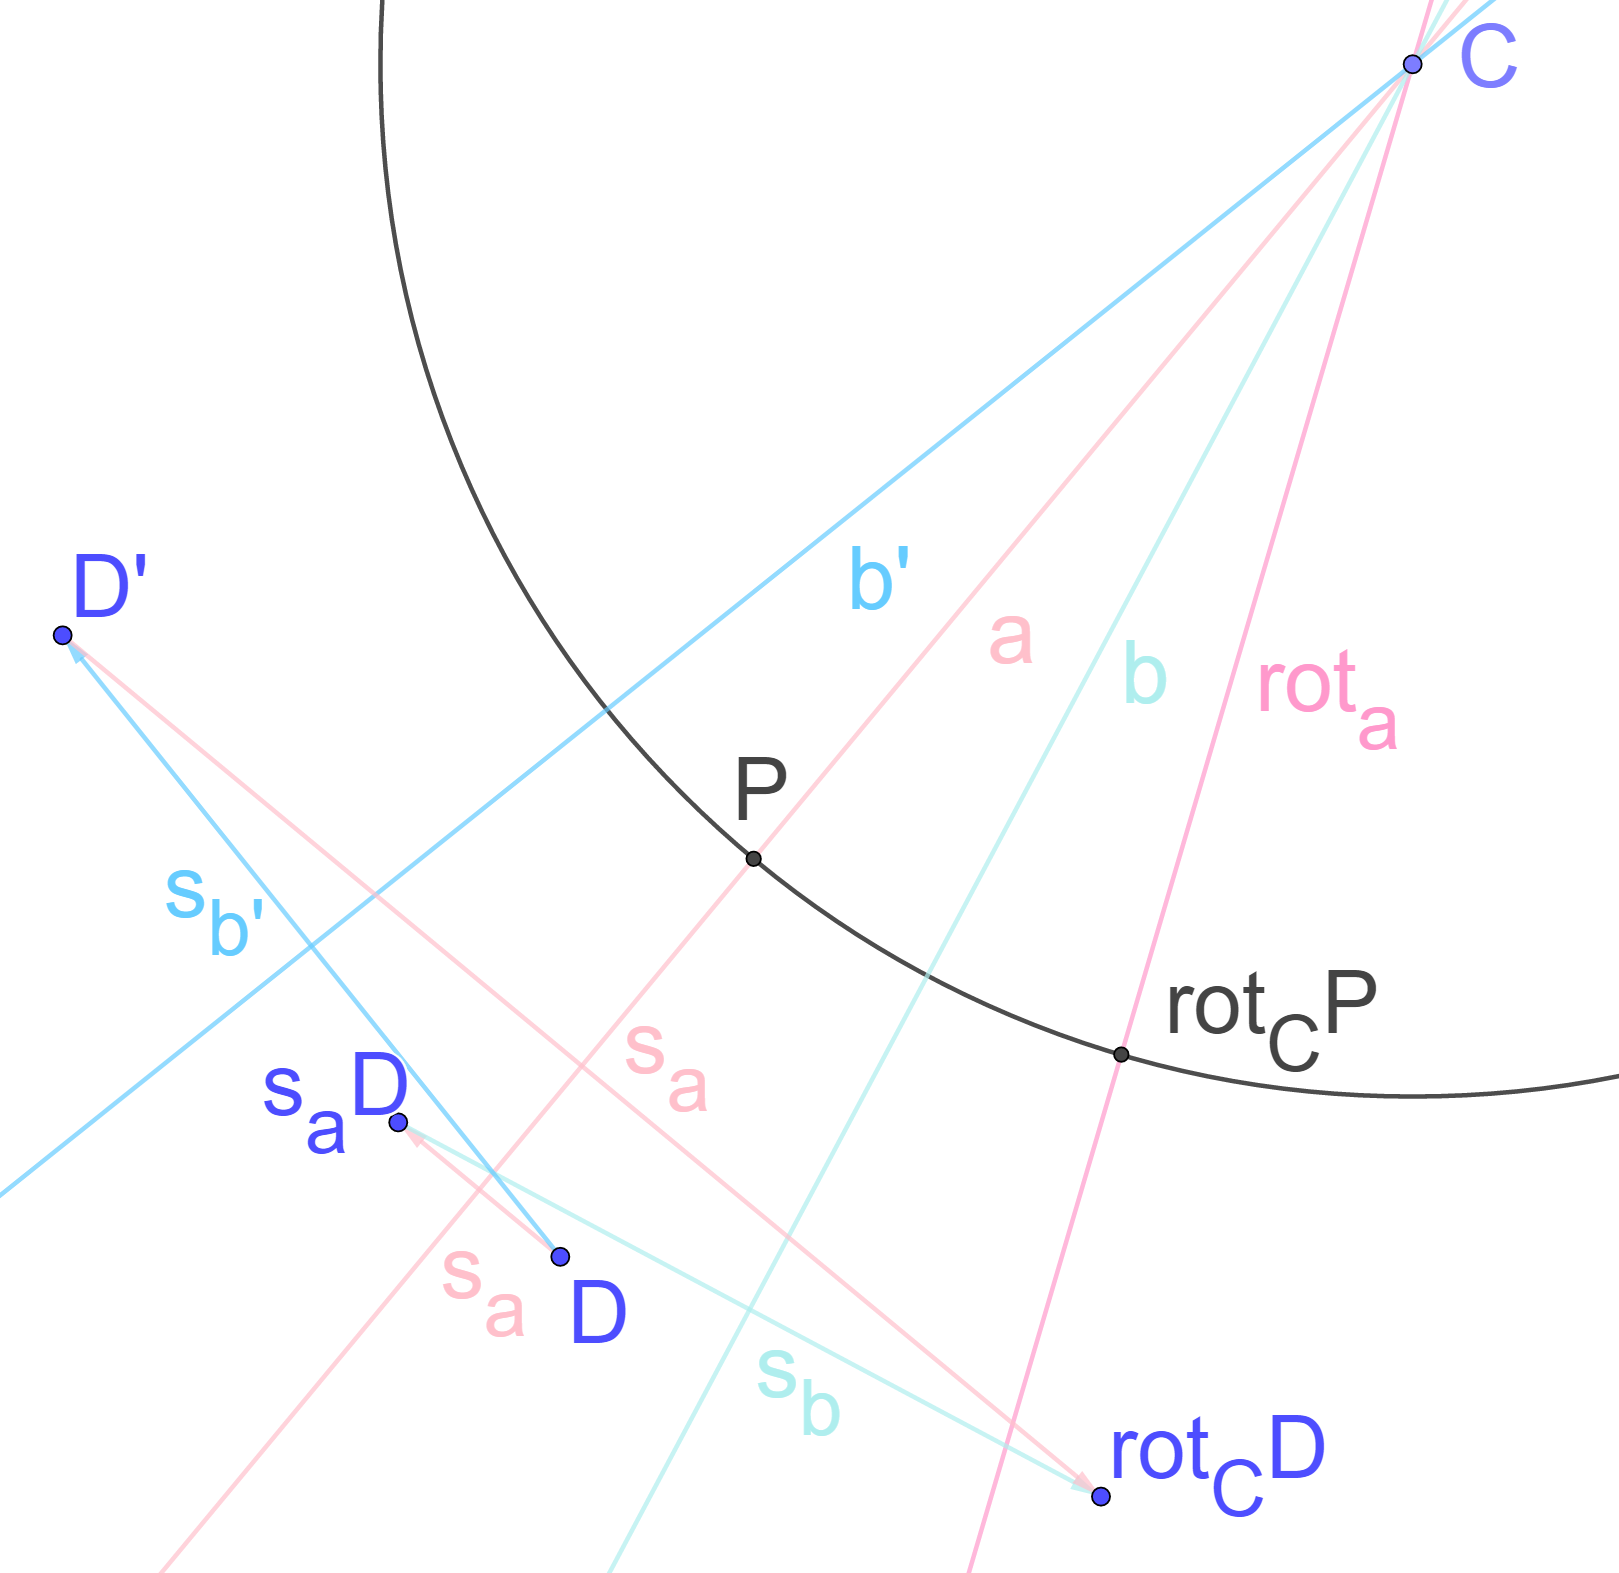
\includegraphics[width=7cm]{figuras/3-9.png}
	\vspace{-1em}
\end{figure}

\ej{3.1} Llamamos $\tau$ una \textbf{traslación} a una isometría que no tiene puntos fijos y deja una recta $c$ invariante, es decir, $\tau(c) = c$. entonces para toda recta $a\perp c$ existen dos rectas $b,b' \perp c$ que cumplen $\tau = \sigma_b\sigma_a = \sigma_a\sigma_{b'}$. Además, si $\tau(l) = l$, entonces $l \parallel c$.

\begin{figure}[H]
	\centering
	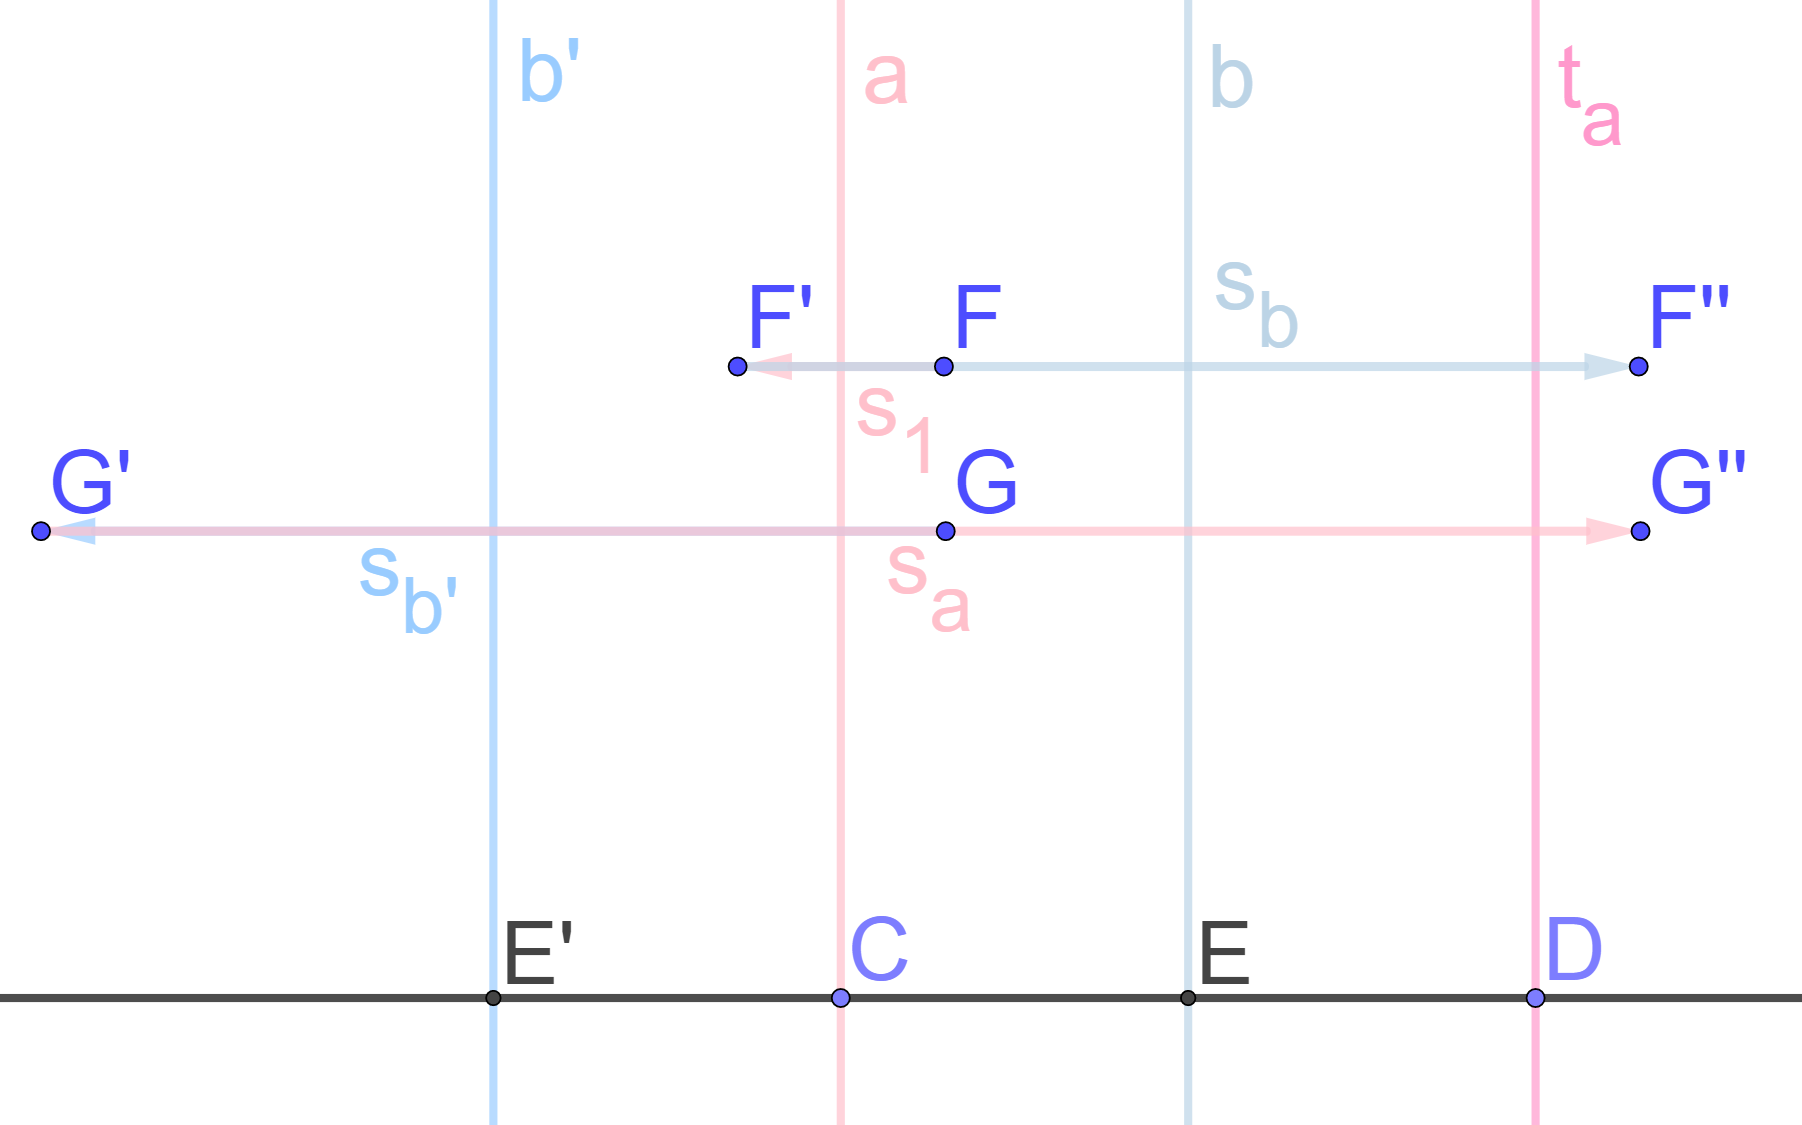
\includegraphics[width=7cm]{figuras/3-1.png}
	\vspace{-1em}
\end{figure}

\ej{3.2} Si $\pazocal{R}_P(\P) = \{g\in \iso(\P) \;|\; g \text{ es} $ 
	\linebreak
	rotación de centro $ P \} \cup \{ \text{id}_\P \}$ entonces
	\begin{itemizex}
		\item Si $a$ es una recta que pasa por $P$, entonces $g^{-1} = \sigma_a g \sigma_a$.
		\item $gh = hg$ para todo $g,h \in \pazocal{R}_P(\P)$.
		\item Para $X \in \P - \{P\}$ y $g(X) = h(X)$ entonces $g = h$.
	\end{itemizex}

\ej{3.3} Si $h$ es una isometría
 	\begin{itemizex}
 	\item Si $g \in \pazocal{R}_P(\P)$ entonces $hgh^{-1} \in \pazocal{R}_{h(P)}(\P)$
 	\item Si $r$ es una recta entonces $h\sigma_rh^{-1} = \sigma_{h(r)}$
	\end{itemizex}

\ej{3.3} Si $a, b$ son rectas en $\P$
	\begin{itemizex}
	 	\item $\sigma_a\sigma_b\sigma_a = \sigma_{a(b)}$
	 	\item $\sigma_a\sigma_b = \sigma_b\sigma_a \iff a \perp b$
	\end{itemizex}

\ejem{3.12} Sean $a,b$ tales que $a\perp_P b$. Entonces la rotación es de 180$^\circ$ y se
llama \textbf{reflexión central} si se denota como $\sigma_P$. Cumple las siguientes propiedades.
	\begin{itemizex}
		\item $\sigma_P\sigma_P= \text{id}_\P$
		\item Para todo $X$, $\sigma_P(X)$ es el único punto que cumple $P = \m[X, \sigma_P(X)]$.
		\item $\sigma_P$ es independiente de la elección de rectas $a\perp b$.
	\end{itemizex}

\tma{3.13} Las rectas $r$ y $\sigma_P(r)$ son paralelas.

\ejem{3.14} Una \textbf{reflexión con deslizamiento} $\phi$ es una composición de una reflexión $\sigma_c$ y una traslación $\tau$: $\phi = \tau\sigma_c$. $\phi$ deja invariante sólo la recta $c$, y no tiene ningún punto invariante.

\tma{3.15} Una isometría solo puede pertenecer a una de las de la tabla, y es una combinación de un número par o impar de reflexiones $\sigma$:

\begin{tabular}{l c c}
	& Con puntos fijos & Sin puntos fijos\\
	par & $\rho$ & $\tau$\\
	impar & $\sigma$ & $\phi$ \\
\end{tabular}


\tma{3.16} Si $g, g'$ son isometrías conjugadas, tienen la misma paridad.






	 
	 